% Template created by Jon Hood

\documentclass[letterpaper, 10pt, twoside]{article}
\usepackage{noto}
\usepackage{fancyhdr}
\usepackage{graphicx}
\usepackage{multirow}
\usepackage[table]{xcolor}
\usepackage[breaklinks=true]{hyperref}
\usepackage[letterpaper, top=1in, bottom=1in, left=1.5in, right=1in, includeheadfoot]{geometry}
\usepackage{wrapfig}

%                Main Variables
\newcommand{\repdate}{\formatdate{24}{9}{2019}}
\def \ProjectName{Security Technical Implementation Guide Qt Viewer}
\def \ProjectAcronym{STIGQter}
\def \ProjectVersion{1.0.0}

%-------------------------------------------------------------------------------
%                Header & Footer Setup
%-------------------------------------------------------------------------------
\pagestyle{fancy}
\lhead[\thepage]{
\includegraphics[height = 2em]{images/STIGQter.pdf}}
\chead{\ProjectName\ --- \ProjectVersion}
\rhead[{
\includegraphics[height = 2em]{images/STIGQter.pdf}}]{\thepage}
\cfoot{\ProjectAcronym\ \ProjectVersion}

\fancypagestyle{blank}
{
	\lhead{}
	\chead{}
	\rhead{}
	\cfoot{}
	\lfoot{}
}

%-------------------------------------------------------------------------------
%                Revisions Table
%-------------------------------------------------------------------------------
\definecolor{STIGQterBlue}{RGB}{30,72,124}
\newcounter{RevisionCounter}
\newenvironment{Revision}{
	\begin{center}
		\begin{tabular}{ | c | c | c | p{23em} | }
			\hline
			\multicolumn{4}{| c |}{\cellcolor{STIGQterBlue}\textbf{\textcolor{white}{Revision History}}} \\
			\hline
			\rowcolor{lightgray}
			\textbf{Date} & \textbf{Revision} & \textbf{Revised By} & \textbf{Reason} \\
			\hline
		}{
	\end{tabular}
\end{center}
}
\newcommand{\RevisionEntry}[3]{\stepcounter{RevisionCounter}
	#1 & \Alph{RevisionCounter} & #2 & #3 \\
	\hline}

%-------------------------------------------------------------------------------
%                Title Page
%-------------------------------------------------------------------------------
\newcommand{\headerlogo}{
	
\includegraphics[width=.3\linewidth]{images/STIGQter.pdf}\\
	\vspace{.5em}
}
\newcommand{\docline}{\textmd{\textbf{STIGQter Installation and Usage Guide\\}}}
\newcommand{\generator}{Generated By: Jon Hood}
\title{
	\headerlogo
	\docline
	\vspace{.5em}
	\normalsize{\generator}
}

\author{Jon Hood}
\date{\repdate}

%-------------------------------------------------------------------------------
%                PDF metadata
%-------------------------------------------------------------------------------
\hypersetup
{
	pdfauthor= (Jon Hood),
	pdftitle =  (STIGQter Installation and Usage Guide)
}

\usepackage{attachfile}
\usepackage[backend=biber]{biblatex}
\usepackage{import}
\usepackage{graphicx}
\usepackage[utf8]{inputenc}
\usepackage{url}
\addbibresource{sources.bib}
\usepackage{setspace}
\usepackage{array}
\usepackage{booktabs}
\newcolumntype{L}{@{}>{\kern\tabcolsep}l<{\kern\tabcolsep}}
\usepackage{colortbl}
\usepackage{xcolor}
\usepackage{textcomp}
\usepackage{outlines}
\usepackage{setspace}
\usepackage{longtable}
\usepackage{enumitem}
\usepackage{listings}
\usepackage{pgfplots}
\usepgfplotslibrary{fillbetween}
\usepackage{datetime}
\newdateformat{changelog}{\THEMONTH/\THEDAY/\THEYEAR}

\lstdefinestyle{CStyle} {language=C}
\lstdefinestyle{CSharpStyle} {language=[Sharp]C}
\lstdefinestyle{PHPStyle} {language=php}
\lstdefinestyle{JavaStyle} {language=java}
\lstdefinestyle{BashStyle} {language=bash}

\lstset{language=C}
\lstset{language=[Sharp]C}
\lstset{language=php}
\lstset{language=java}
\lstset{language=bash}

\newcolumntype{L}[1]{>{\raggedright\let\newline\\\arraybackslash\hspace{0pt}}m{#1}}
\newcolumntype{C}[1]{>{\centering\let\newline\\\arraybackslash\hspace{0pt}}m{#1}}
\newcolumntype{R}[1]{>{\raggedleft\let\newline\\\arraybackslash\hspace{0pt}}m{#1}}

%start the document
\begin{document}

%generate a title page
\thispagestyle{blank}
\maketitle
\newpage

\thispagestyle{blank}
This page intentionally left blank for 2-sided printing compatibility.
\newpage

%tell the page counter to restart
\setcounter{page}{1}
\pagenumbering{roman} %use lowercase Roman numerals for page numbers

%Revision History page
\begin{Revision}
\RevisionEntry{\date{\changelog\formatdate{29}{10}{2019}}}{Jon Hood}{Initial Release of Documentation}

\end{Revision}
\newpage

%generate a table of contents
\setcounter{tocdepth}{2}
\tableofcontents
\cleardoublepage % go to next right-side page

%reset the page counter for the regular pages
\setcounter{page}{1}
\doublespacing
\pagenumbering{arabic} %use standard numbers for the page number

\section{Background}
STIGViewer has been the DISA-provided tool of choice for creating STIG Checklists (CKL) and Continuous Moniitoring Risk Scoring (CMRS) reports for eMASS. It is a solid tool, stable, and unfortunately closed-source. STIGQter attempts to recreate the features of STIGViewer in an open and extensible way. The goal of STIGQter is to abide by free and open source principles so that it may be incorporated and distributed freely in any operating system.

\section{Starting Up}
\begin{wrapfigure}{R}{0.6\textwidth}
	\centering
	\vspace{-70pt}
	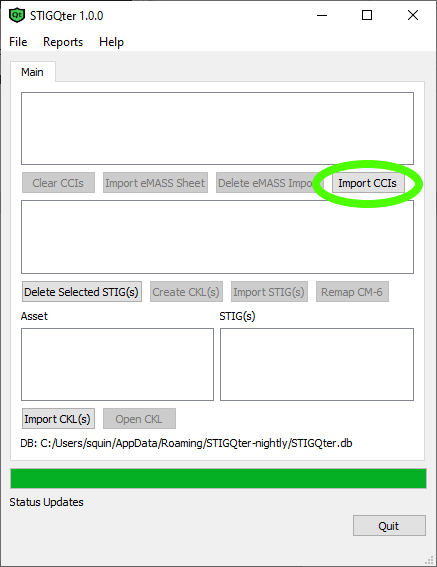
\includegraphics[width=0.59\textwidth]{images/main-01.png}
	\caption{Starting Main Interface}
	\vspace{-10pt}
	\label{fig:importccis}
\end{wrapfigure}
To use STIGQter, you will need to index the set of RMF Controls from NIST, the set of CCIs from DISA, and obtain the relevant STIGs for your system.

\subsection{Indexing Controls and CCIs}
The first step in using STIGQter is to index the latest RMF Controls and CCIs from NIST and Cyber.mil respectively. To do this, click the ``Import CCIs'' button (Figure~\ref{fig:importccis}).

STIGQter will index the base CCIs associated with NIST 800-53 Revision 4 automatically. When done, it will download the latest CCI list from DISA to incorporate the latest DoD modifications. These CCIs form the base units of validation in eMASS: issues are recorded at the CCI level and roll up to the Control level.

\subsection{Indexing STIGs}

\clearpage
\printbibliography

\end{document}
